
This appendix will present the method used in this work to obtain the magnitude and phase response of the actuation system for a given sinusoidal input.

The model block diagram is shown in Figure \ref{fig:B_SimulinkModel}. In the frequency response test, the sinusoidal surface command is inserted in signal \textit{$SurfacePositionCmd\_(deg)$} and the output is the surface position in degrees represented by the signal \textit{$SurfacePosition\_(deg)$}.

\begin{figure}[H]
	\centering
	\centerline{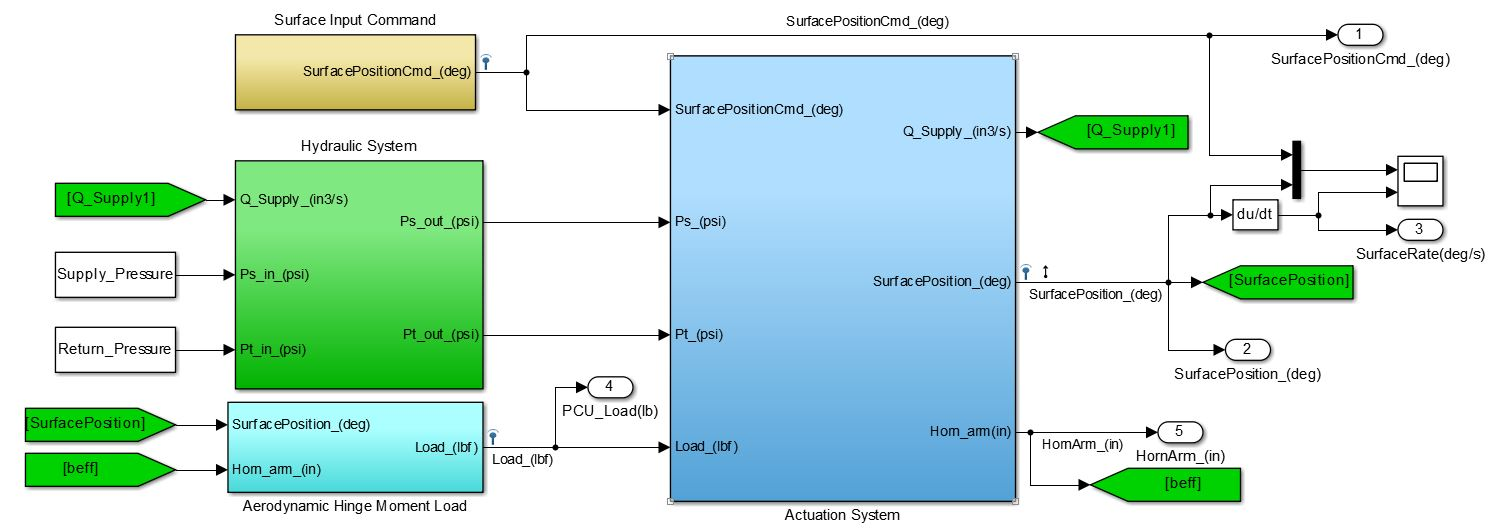
\includegraphics[width=1.1\textwidth]{Figuras/3.ActuationSystemModel/3-Model.jpg}}
	\caption{Actuation System and Interfaces Simulink Model}
	\label{fig:B_SimulinkModel}
\end{figure}

Since the actuation system is non-linear, the output signal may contain components in frequencies different from the one of the input. Figure   shows an example of a 20 Hz sine surface command with an amplitude of 0.5 degrees. The figure also presents the correspondent output signal and it is possible to observe that the output is not a pure sine and therefore was distorted by the system. 

\begin{figure}[H]
	\centering
	\centerline{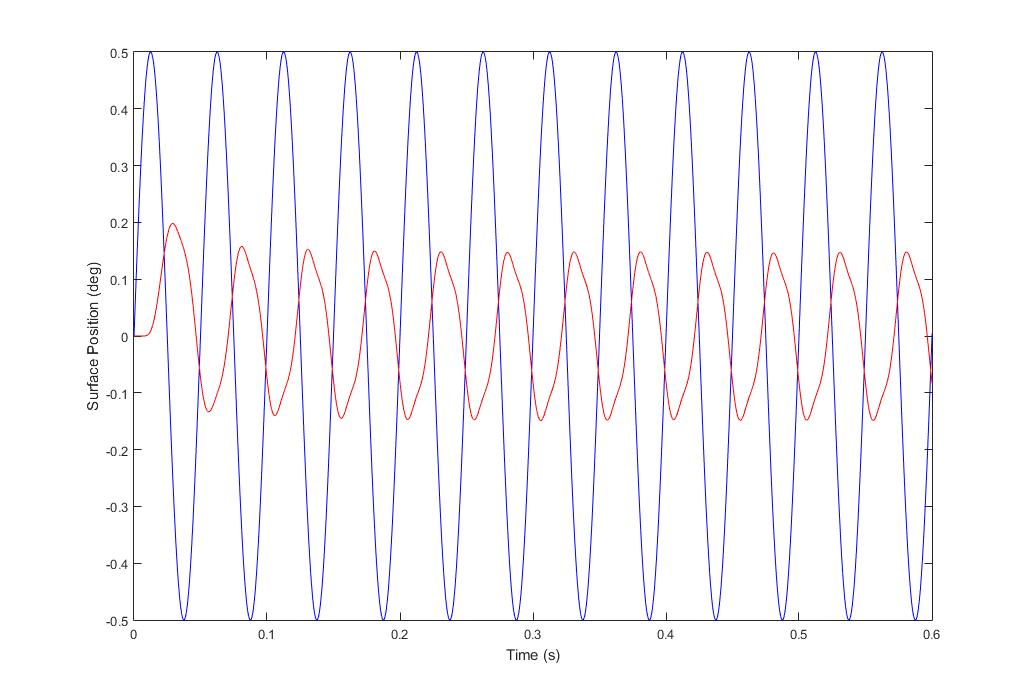
\includegraphics[width=1.1\textwidth]{Figuras/B.NonlinearFR/20HzTimeResponse.jpg}}
	\caption{System Output for a 20Hz sine input signal}
	\label{fig:B_InputOutput}
\end{figure}

Hence, the system output can be a linear combination of sine signals of different frequencies and for this reason a method to find the magnitude and phase of the system transfer function needs to be defined. The Total Harmonic distortion (THD) of a signals quantifies the relative power between the fundamental frequency and the harmonics and it can be used as a measure of how non-linear is the system. 

Figure \ref{fig:B_Spectrum} shows the frequency power spectrum of the system output presented previously. In this case, the power of the fundamental frequency is -18.54 dB and the Total Harmonic Distortion (THD) is -31.8 dB or 2.5\%.

\begin{figure}[H]
	\centering
	\centerline{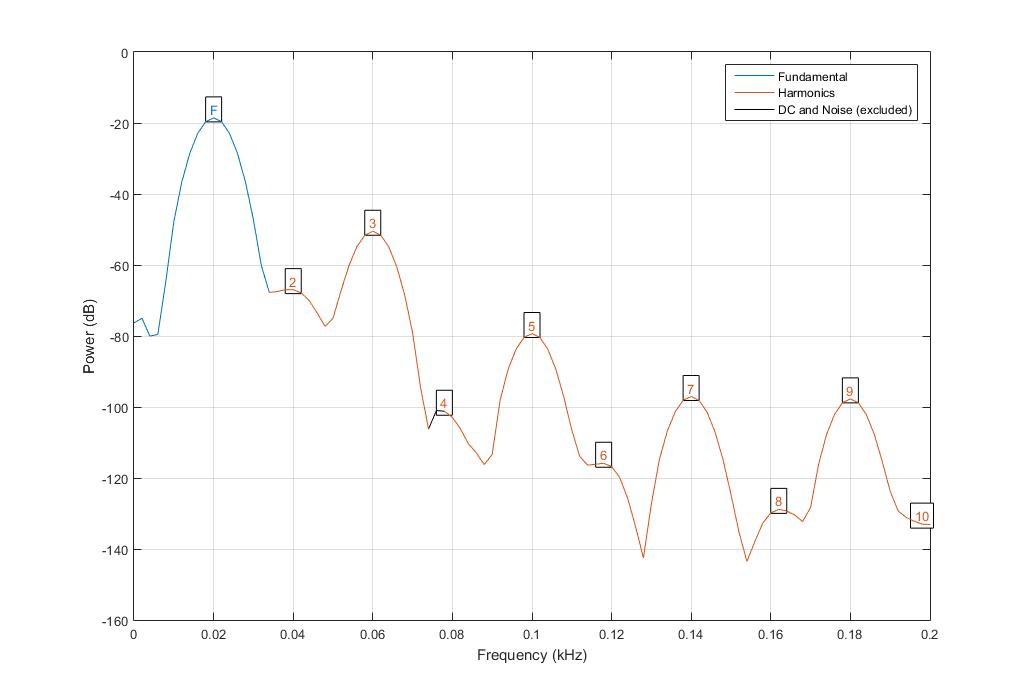
\includegraphics[width=1.1\textwidth]{Figuras/B.NonlinearFR/THD20HZ.jpg}}
	\caption{System Output for a 20Hz sine input signal}
	\label{fig:B_Spectrum}
\end{figure}

In this work it was considered an acceptable THD of 10\% or lower. In this cases, the system magnitude and phase responses were calculated considering only the component of the fundamental frequency in the output signal of the system.

Table \ref{table:B_THD} below shows the THD in each evaluated frequency for a PD controller with $K_P=40$ and $K_D=0.7$.

\begin{table}[H]
	\captionof{table}{THD values of a PD controller frequency response}
	\label{table:B_THD}
	\centering
	\resizebox{14cm}{!} {
		\begin{tabular}{|c|c|c|c|c|c|}
			\hline
			Frequency (Hz)  & THD (\%) & Frequency (Hz) & THD (\%) & Frequency (Hz) & THD (\%) \\ \hline
			$0.1$ & $6.21$  & $8$  & $3.18$ & $17$ & $5.29$ \\ \hline
			$0.5$ & $4.61$  & $9$  & $3.51$ & $18$ & $4.11$ \\ \hline
			$1$   & $4.05$  & $10$ & $2.72$ & $19$ & $3.15$ \\ \hline
			$2$   & $4.90$  & $11$ & $2.38$ & $20$ & $2.46$	\\ \hline
			$3$   & $2.98$  & $12$ & $2.58$ & $25$ & $0.99$	\\ \hline
			$4$   & $2.83$  & $13$ & $3.63$ & $30$ & $0.42$	\\ \hline	
			$5$   & $2.76$  & $14$ & $6.09$ & $35$ & $0.20$	\\ \hline	
			$6$   & $2.76$  & $15$ & $7.83$ &      &  		\\ \hline	
			$7$   & $2.89$  & $16$ & $6.82$ &      &  		\\ \hline	
	\end{tabular}}
\end{table}

The table shows that the maximum value of the THD is 7.83\% at 15 Hz, therefore the proposed methodology was applied for all frequencies. This was also considered for the four types of controllers evaluated in this work (P, PI, PD and PID) since the controllers have linear transfer functions and should not interfere in the spectrum of the output signal. 




